% This must be in the first 5 lines to tell arXiv to use pdfLaTeX, which is strongly recommended.
\pdfoutput=1
% In particular, the hyperref package requires pdfLaTeX in order to break URLs across lines.

\documentclass[11pt]{article}

% Remove the "review" option to generate the final version.
\usepackage{acl}
\usepackage{graphicx}
\graphicspath{ {./narrative_eye_tracking_analysis/images/} }
% Standard package includes
\usepackage{times}
\usepackage{latexsym}
\usepackage{hyperref}
% For proper rendering and hyphenation of words containing Latin characters (including in bib files)
\usepackage[T1]{fontenc}
% For Vietnamese characters
% \usepackage[T5]{fontenc}
% See https://www.latex-project.org/help/documentation/encguide.pdf for other character sets

% This assumes your files are encoded as UTF8
\usepackage[utf8]{inputenc}

% This is not strictly necessary, and may be commented out,
% but it will improve the layout of the manuscript,
% and will typically save some space.
\usepackage{microtype}
\usepackage{float}

% If the title and author information does not fit in the area allocated, uncomment the following
%
%\setlength\titlebox{<dim>}
%
% and set <dim> to something 5cm or larger.

\title{An Analysis of Reader Engagement in Literary Fiction through Eye Tracking}


\author{Rose Neis \\
  University of Minnesota  \\
  \texttt{neis@umn.edu}
  \And
  Karin de Langis \\
  University of Minnesota\\
  \texttt{dento019@umn.edu} \\
  \AND
  Zae Myung Kim \\
  University of Minnesota\\
  \texttt{kim01756@umn.edu}
  \And
  Dongyeop Kang \\
  University of Minnesota\\
  \texttt{dongyeop@umn.edu} \\
  }

\begin{document}
\pagenumbering{arabic}
\maketitle

\begin{abstract}
Capturing readers' engagement in fiction is a challenging but important aspect of narrative understanding. In this study, we collected 23 readers’ reactions to 2 short stories through eye tracking, sentence-level annotations, and an overall engagement scale survey. Our aim is to analyze the significance of various qualities of the text in predicting how engaging a reader is likely to find it. As enjoyment of fiction is highly contextual, we will also investigate individual differences in our data. Furthering our understanding of what captivates readers in fiction will help better inform models used in creative narrative generation and collaborative writing tools.
\end{abstract}
\section{Introduction}
The question of reader engagement in fiction has been studied in the psychology field for decades, with some of the foundational theoretical work from Gerrig on Transportation Theory \citep{gerrig_1993} paving the way for more recent theoretical frameworks and experimental setups, notably the work by Green et al. \citep{Green2004,green_brock_kaufman_2006}. There have been several more experimental setups in recent years. 

However, as Arthur Jacobs emphasized in his article, "Towards a neurocognitive poetics model of literary reading", the samples normally collected are small and not enough to compensate for individual differences in reading patterns due to reader context and other situational factors \citep{willems_2015}. In order to help close the experimental gap, one contribution of this study is to provide the computational community with a data set of reader reactions to natural stories, which Jacobs refers to as "hot" experimental research.

In his framework laid out in the same article, he proposed two modes of reading: one fast track --- 'immersion' and one slow --- 'aesthetic trajectory'. The former is proposed to be brought on by things like familiarity, suspense, sympathy, and vicarious hope; whereas the latter is a more reflective and connected mode brought on by aesthetic appreciation and unfamiliar situations. Although this is difficult to ascertain at the lexical level, we compared our findings to the extent that we could to this model.

In a 2009 study, a pair of researchers narrowed down the salient aspects of reader engagement, building off of Green's transportation framework to create media engagement scale \citep{busselle2009}, which we modified slightly to gage overall interest in the stories used in our study. In addition, in order to obtain more granular information, we used these aspects to design an annotation task that would provide sentence-level feedback. Using visualizations and linear mixed models, we explored textual features that had an impact on engagement and dwell time across readers.

\section{Related Research}
There have been several eye tracking and fMRI studies in the area of reader interest (a few are shown in \autoref{tab:first}). We compared our findings with a select few existing experiments as well as Jacobs' framework. One 13-participant study showed that words in enactive passages had on average longer fixation durations and dwell times \citep{Magyari2020}. Based on survey responses, the authors hypothesize that in the enactive texts, the ease of imagery contributes to greater involvement in imagination and results in an overall slower reading speed. An fMRI study found valence and arousal scores as good predictors of overall emotional experience of the reader \citep{HSU201596}. 


\begin{table*}[h]
\centering
\begin{tabular}{|c|c|c|c|c|c|c|}
\hline
& \textbf{Ours} & \textbf{Kunz et al.} & \textbf{Mangen et al.} & \textbf{Hsu et al.} & \textbf{Mak et al.} & \textbf{Maslej et al.} \\
\hline
\multicolumn{7}{|l|}{\textbf{Data gathered}}\\\hline
Eye tracking & x & x & x &  & x &  \\\hline
Saccade angle &  & x & x &  &  & \\\hline
fMRI &  &  &  & x &  & \\\hline
Engagement survey & x & x & x &  & x & x\\\hline
Engagement annotation & x &  &  & x &  & \\\hline
\multicolumn{7}{|l|}{\textbf{Textual features extracted}}\\\hline
Emotional arc & x &  &  &  &  & \\\hline
Lexical categories & x &  &  & x &  & x\\\hline
Description category &  &  & x &  &  & \\\hline

\end{tabular}
\caption{Comparison between our study and other similar experiments.}
\label{tab:first}
\end{table*}

\section{Research questions}

\subsection{RQ1: Does absorption in a story lead to longer gaze durations?}
\label{subsection:rq1}

To answer this question, we looked at how well “Present” highlights (i.e. transported) correlate with faster reading and “Connected” and “Curious” highlights with slower reading to see if there is a relationship between dwell time and different modes of reading -- one being immersed and the other more reflective. We also looked at whether features related to a more affective reading mode lead to higher dwell times as Jacobs predicts.

\subsection{RQ2: How much is engagement dependent on reader context vs. linguistic features?}
\label{subsection:rq2}

In order to address this question, we evaluated how well the features we extracted could predict whether a sentence was highlighted by readers.

\subsection{RQ3: Are dwell time patterns consistent across readers?}
\label{subsection:rq3}

We scaled dwell times per participant and evaluated the pattern over the story to see if dwell times increased and decreased in the same areas of the story for different readers.

\section{Methods}

\subsection{Participant study}

The study asked 31 English speakers (17 female, 11 male, 3 other, 23 native English speakers, average age: 26) were asked to read two short stories by Anton Chekhov while their eyes were tracked, and then answer an engagement scale survey:

\begin{itemize}
  \item I was curious about what would happen next. (+)
  \item The story affected me emotionally. (+)
  \item While reading my body was in the room, but my mind was inside the world created by the story. (+)
  \item At times while reading, I wanted to know what the writer\'s intentions were. (+)
  \item While reading, when a main character succeeded, I felt happy, and when they suffered in some way, I felt sad. (+)
  \item The characters were alive in my imagination. (+)
  \item I found my mind wandering while reading the story. (-)
  \item I could vividly imagine the scenes in the story. (+)
  \item At points, I had a hard time making sense of what was going on in the story (-)
\end{itemize}

After reading through both stories, they completed a highlighting exercise where they highlighted areas according to the following categories:

\begin{itemize}
  \item Present: Able to vividly picture the scene in the story
  \item Confused
  \item Curious: Curious about what will happen next
  \item Connected: Connected to the character; able to identify with them or feel their emotions
  \item Other: Enjoyed it for a different reason
\end{itemize}

Due to calibration issues, 8 samples were discarded, leaving 23 (13 female, 8 male, 2 other, 17 native English speakers, average age: 28).

The eye tracking results were drift corrected and interest area reports were exported using words as interest areas. Outliers for dwell time were removed using the inner quartile range method (1.7\% of the data). The data was aggregated to the sentence level and dwell time values were normalized by sentence character count. To handle missing data, null values for the eye tracking features were filled with the average of the 5 nearest sentences (5.7\% of all sentences read across participants).

\begin{figure*}[h]
  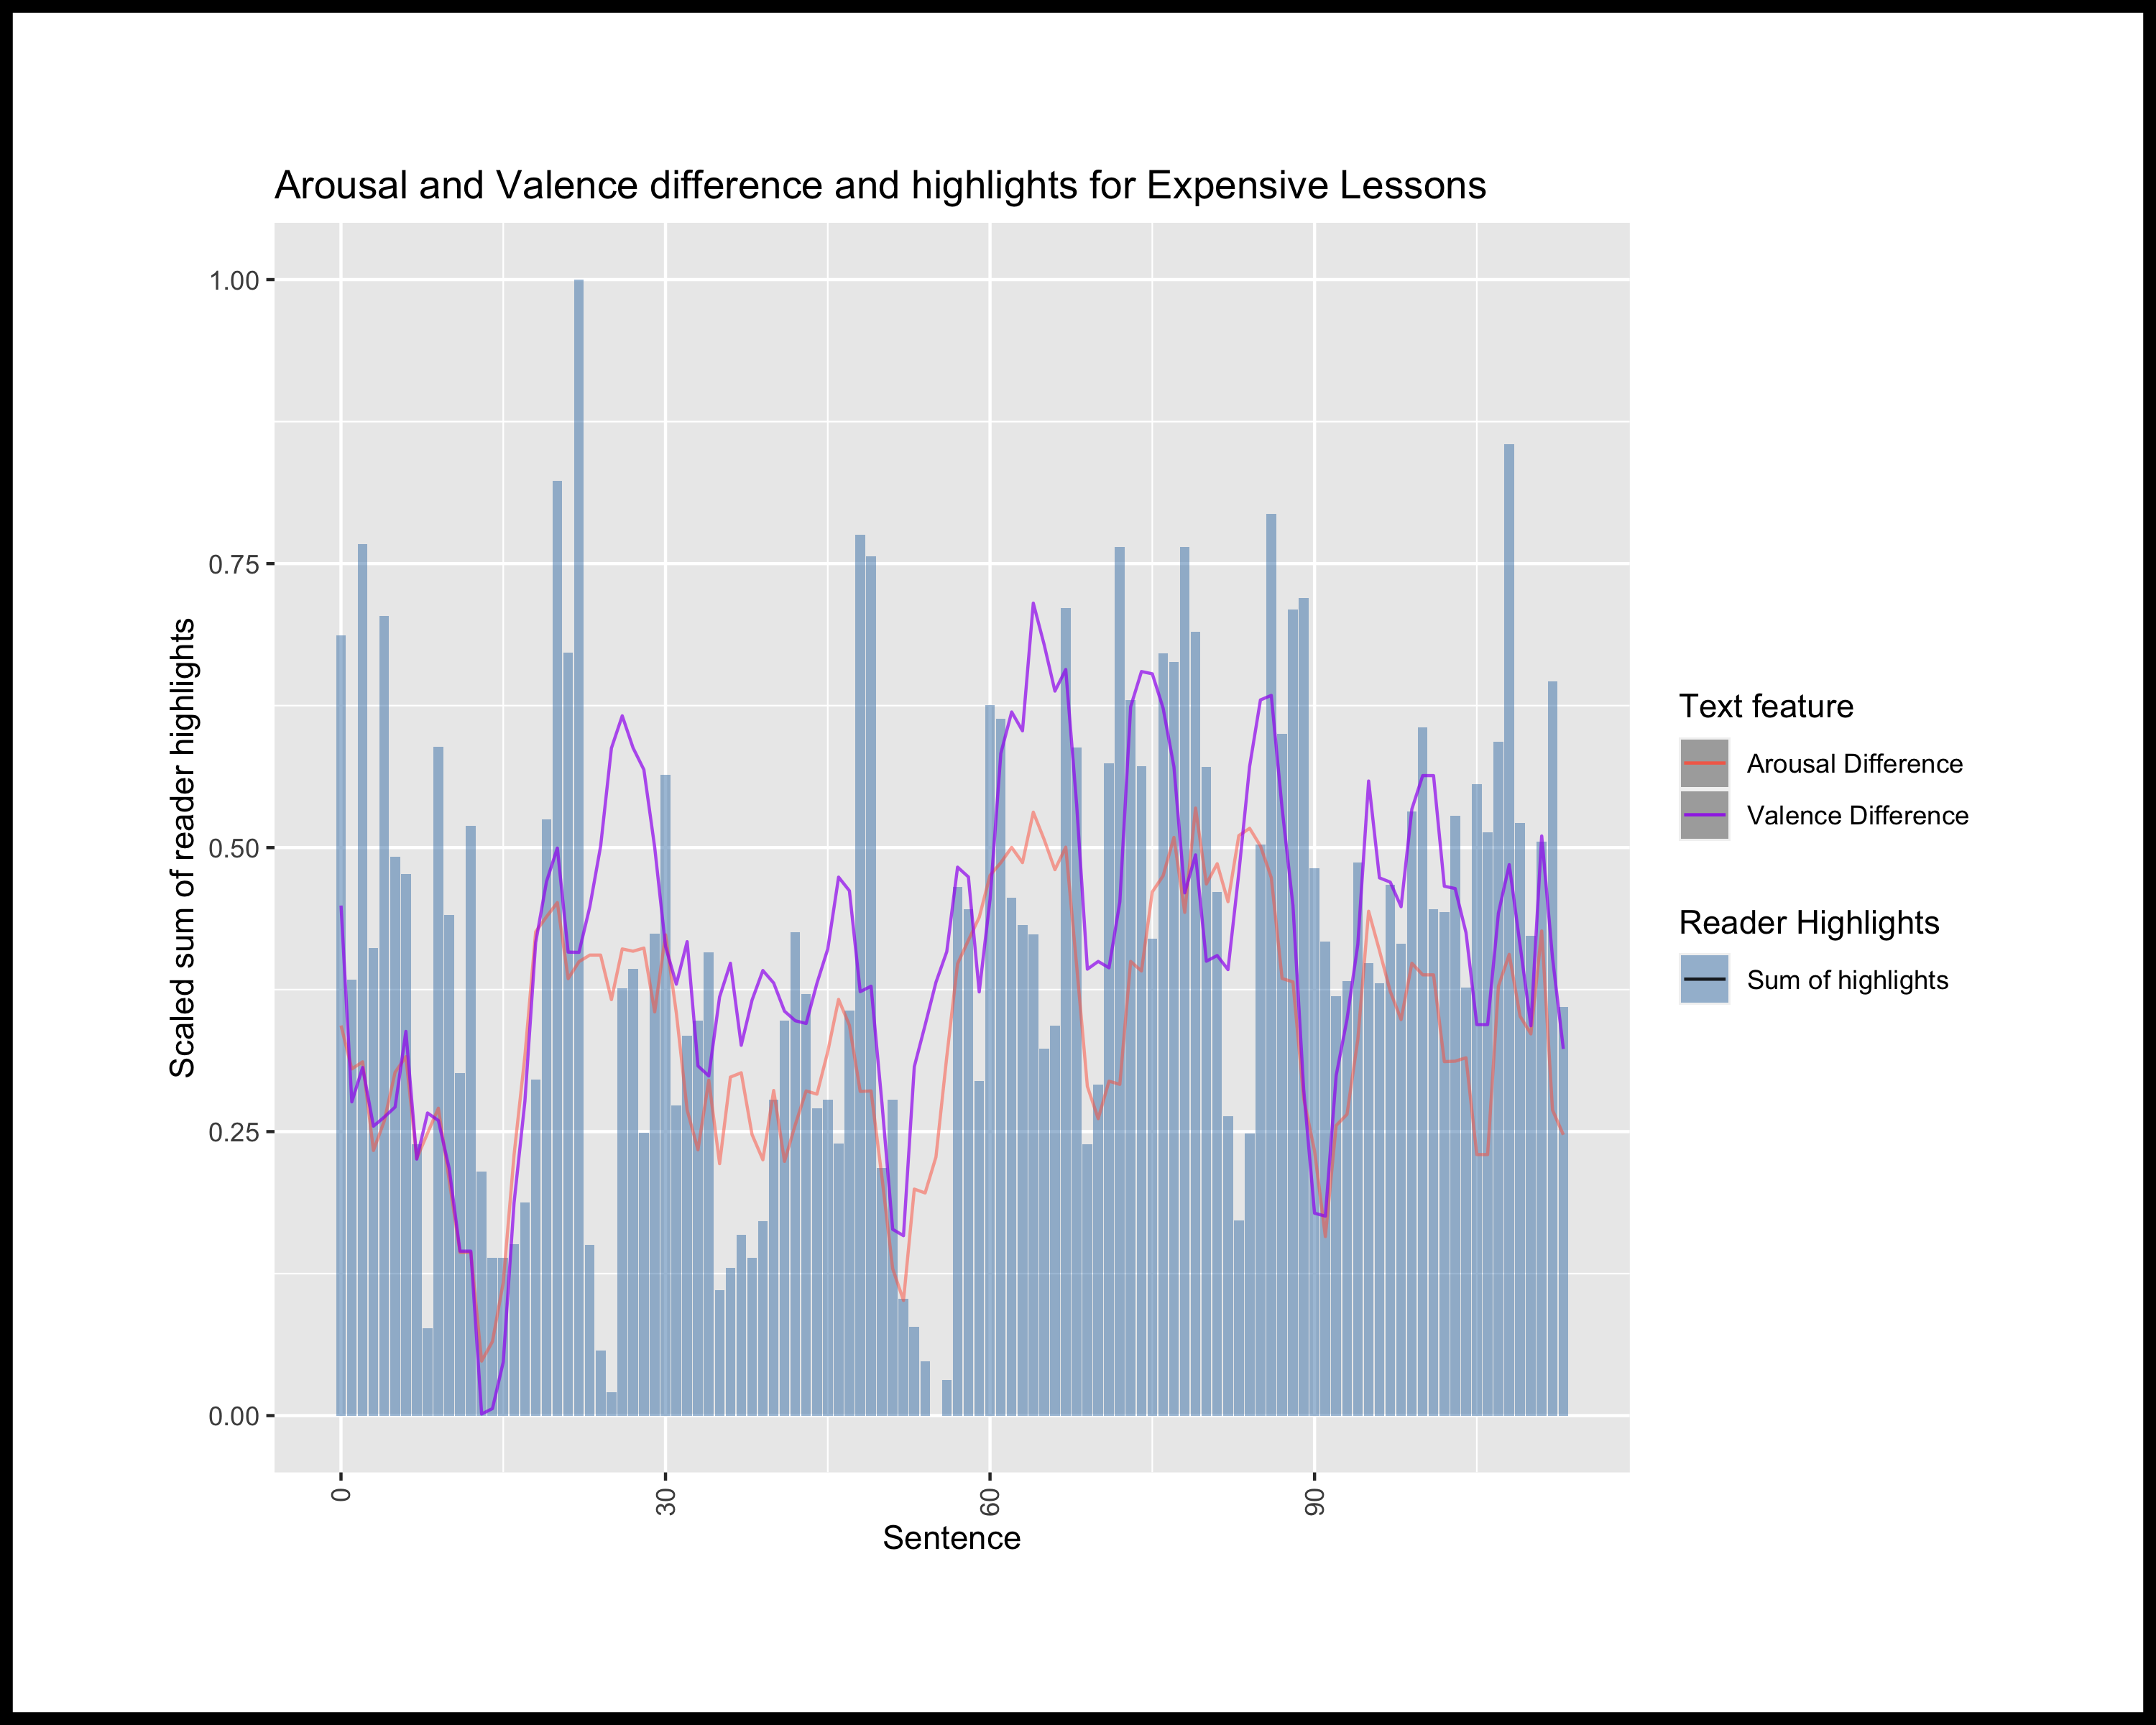
\includegraphics[height=6cm]{el_highlights_val_arousal}
  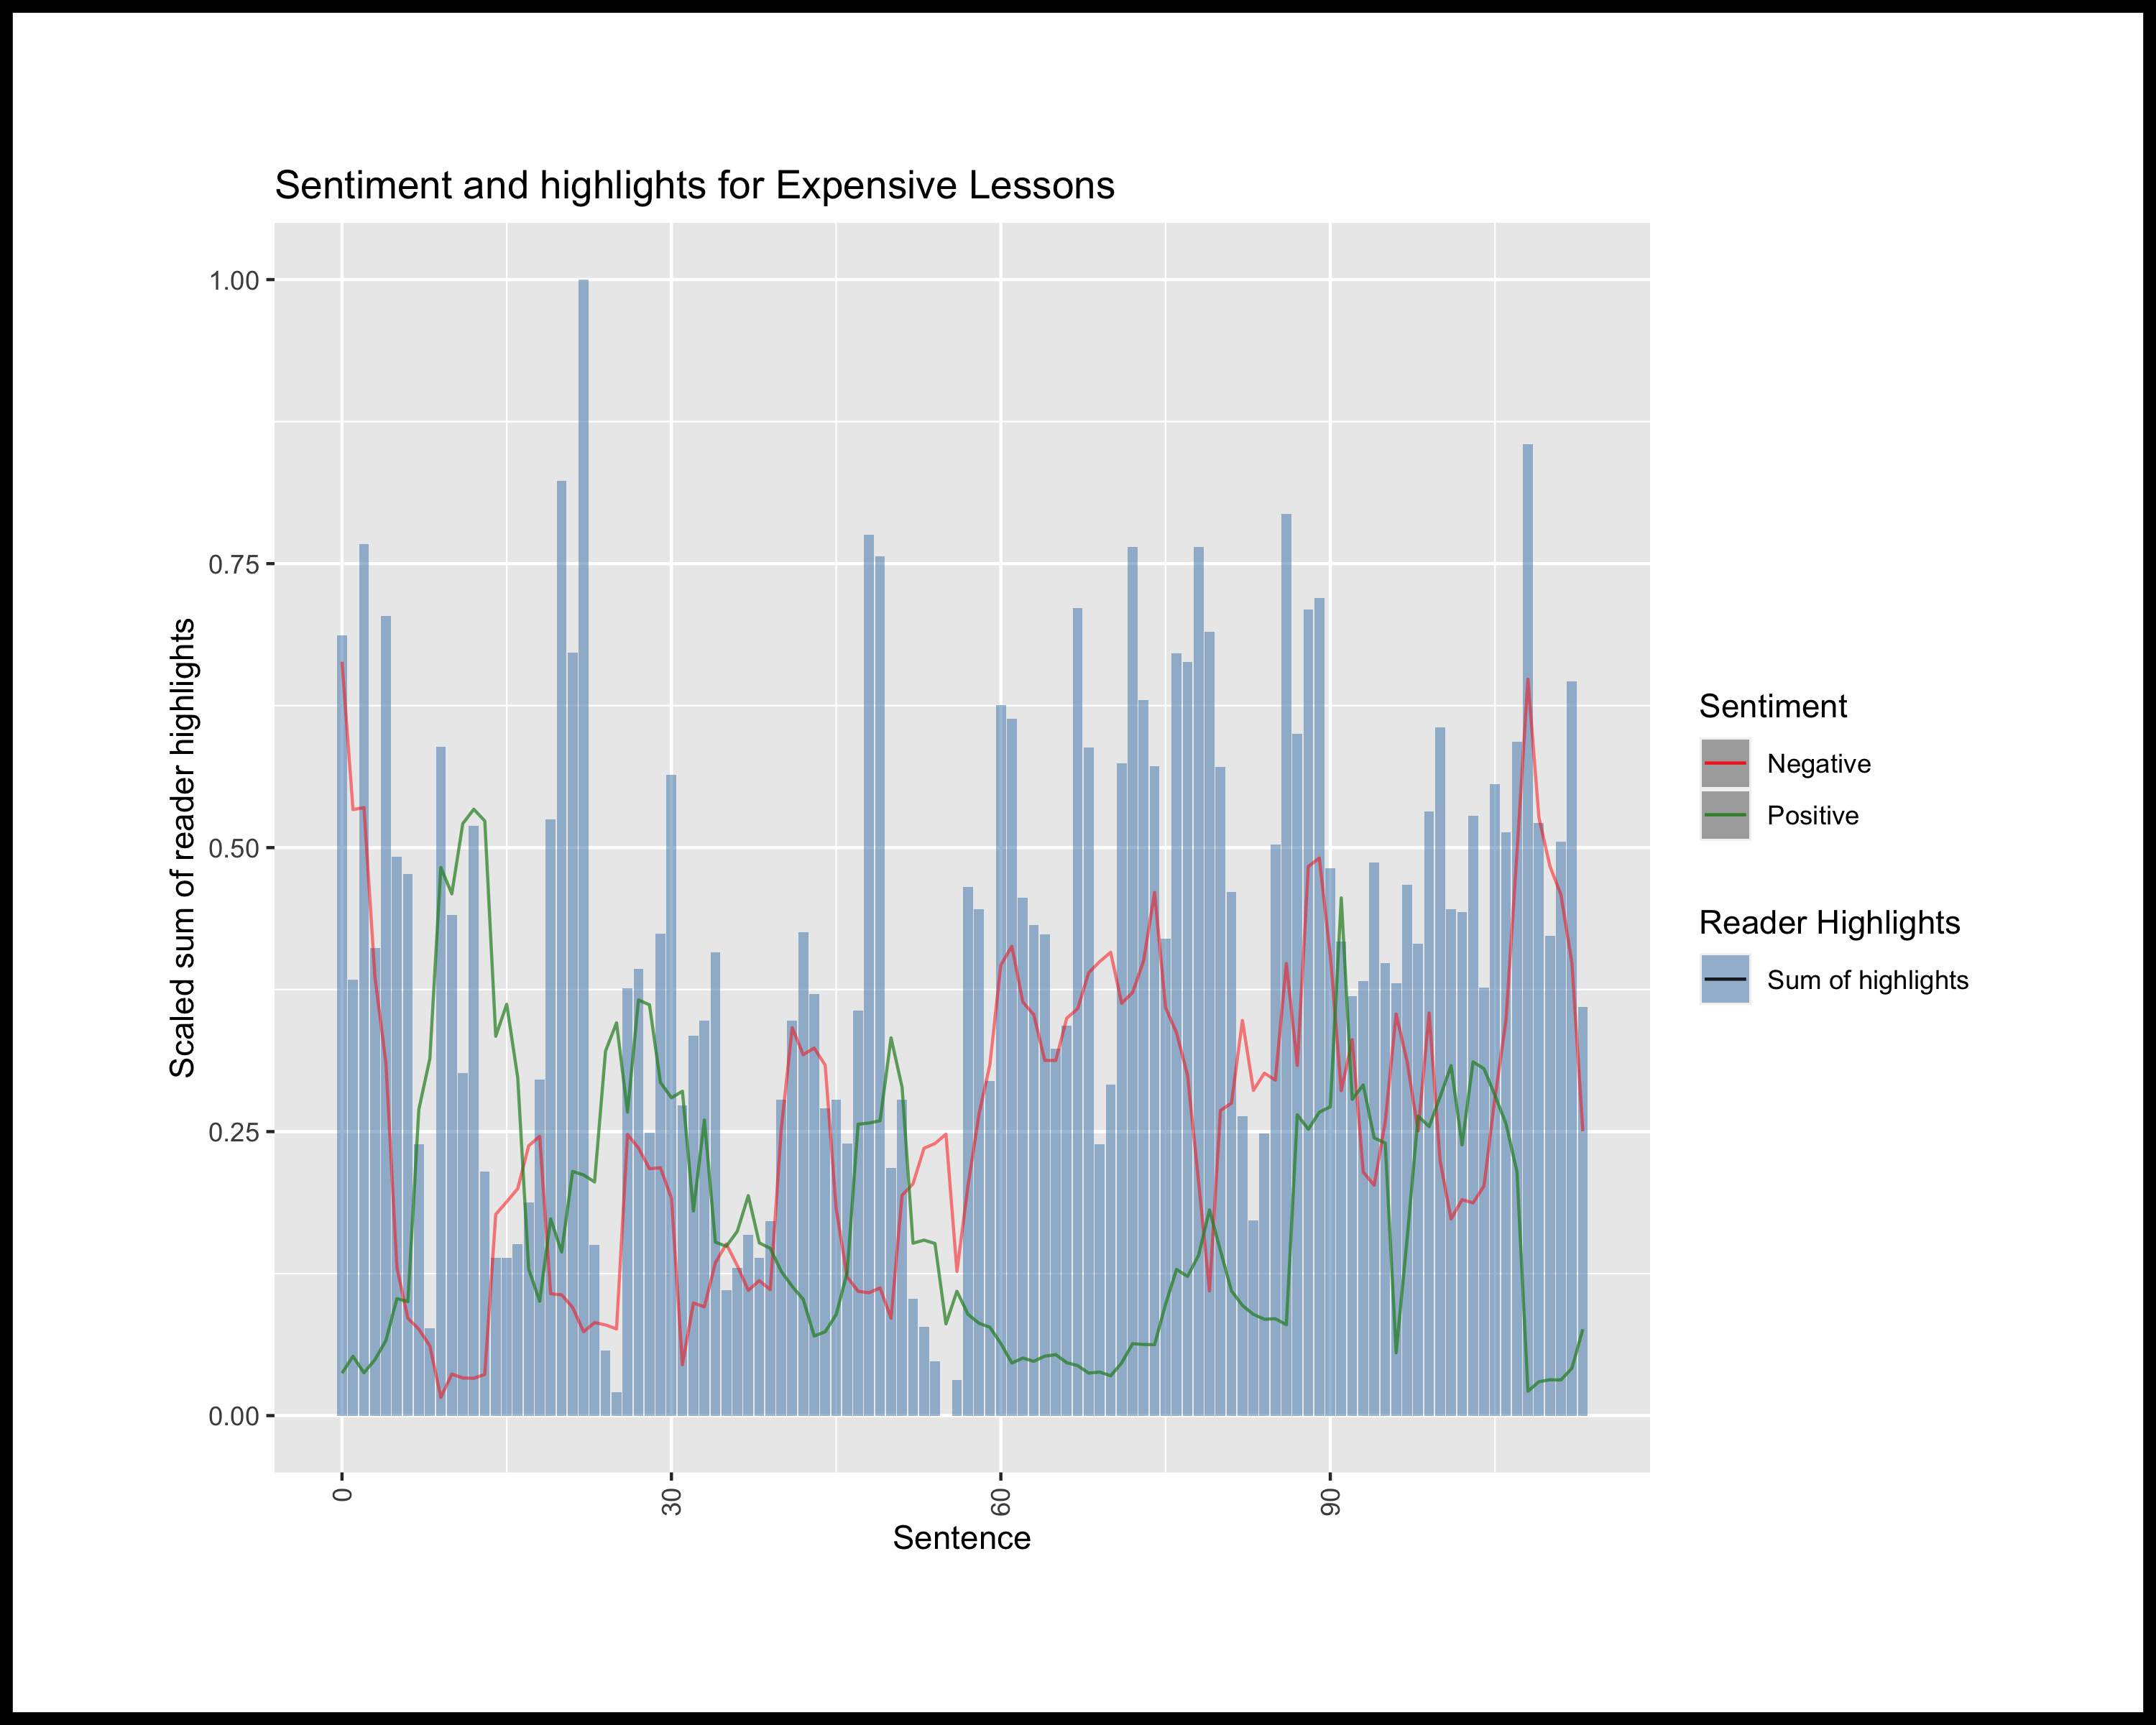
\includegraphics[height=6cm]{el_highlights_sentiment}
  \caption{Highlights and features.}
\end{figure*}

\subsection{Linguistic and discourse features}

We extracted the following features from the stories to create sentence-level predictors: sentiment scores using the RoBERTa sentiment base model \footnote{https://huggingface.co/cardiffnlp/twitter-roberta-base-sentiment}, emotion categories using the DistilRoBERTa emotion base model \footnote{https://huggingface.co/j-hartmann/emotion-english-distilroberta-base}, concreteness scores from the Brysbaert corpus \citep{brysbaert2014}, valence and arousal from the NRC-VAD corpus \citep{valence_arousal_dominance_2013}, word frequency from the subtlex corpus \citep{Brysbaert_2015}, and average word length.

\section{Limitations}

There are a few issues with the data that should be mentioned. Since the participants were asked to read two stories in a row, it is best to make sure there is a balance in which story is read first. However, our data ended up with a skew towards one story (Expensive Lessons: 16, Schoolmistress: 7), which may affect level of attention for the second story. 

In addition, the stories did not receive high scores on average in the engagement survey. On a scale from 0-4, Expensive Lessons got an average of 2.09 and Schoolmistress averaged 1.92. Ideally, stories used for such studies should be more widely popular in order to make absorption more likely. Perhaps in part due to the low average score, the highlighting data is sparse, making it difficult to find relationships between dwell time and engagement categories.

\section{Results}

\begin{table*}[h]
\centering
\begin{tabular}{|l|r|r|r|r|r|r|}
\hline
& Estimate & Std. Error & df & t value & $Pr(>|t|)$ & Sig. \\
\hline
(Intercept) & -0.05352 & 0.07761 & 296.542 & -0.690 & 0.49102 & \\
character count & 0.16092 & 0.03710 & 7023.920 & 4.337 & $1.46 \times 10^{-5}$ & $\ast\ast\ast$ \\
word frequency & 0.07002 & 0.04102 & 6769.055 & 1.707 & 0.08786 & . \\
positive & 0.03786 & 0.02241 & 7118.596 & 1.690 & 0.09116 & . \\
negative & 0.09271 & 0.02044 & 7085.737 & 4.536 & $5.84 \times 10^{-6}$ & $\ast\ast\ast$ \\
concreteness & 0.01938 & 0.01366 & 6380.945 & 1.419 & 0.15598 & \\
valence mean & 0.11482 & 0.04536 & 7118.133 & 2.531 & 0.01139 & $\ast$ \\
arousal mean & -0.02189 & 0.05424 & 7118.401 & -0.404 & 0.68656 & \\
valence span & 0.10988 & 0.02647 & 7117.824 & 4.151 & $3.35 \times 10^{-5}$ & $\ast\ast\ast$ \\
arousal span & 0.10874 & 0.03210 & 7057.269 & 3.388 & 0.00071 & $\ast\ast\ast$ \\
surprise & 0.08417 & 0.02558 & 6987.261 & 3.290 & 0.00101 & $\ast\ast$ \\
disgust & 0.02947 & 0.01563 & 7115.526 & 1.885 & 0.05949 & . \\
\hline
\end{tabular}
\caption{Fixed Effects for predicting proportion of sentence highlighted}
\label{tab:second}
\end{table*}

\begin{table*}[h]
  \centering
  \begin{tabular}{|l|r|r|r|r|r|r|}
  \hline
  & Estimate & Std. Error & df & t value & $Pr(>|t|)$ & Sig. \\
  \hline
  (Intercept) & 0.1010 & 0.0245 & 84.24 & 4.129 & $8.53 \times 10^{-5}$ & $\ast\ast\ast$ \\
  word frequency & 0.1877 & 0.0124 & 7105 & 15.086 & $< 2 \times 10^{-16}$ & $\ast\ast\ast$ \\
  positive & 0.01352 & 0.006773 & 7120 & 1.996 & 0.045920 & $\ast$ \\
  negative & 0.009938 & 0.006108 & 7120 & 1.627 & 0.103740 & \\
  concreteness & 0.01515 & 0.004112 & 7077 & 3.683 & 0.000232 & $\ast\ast\ast$ \\
  valence mean & -0.06013 & 0.01367 & 7120 & -4.399 & $1.10 \times 10^{-5}$ & $\ast\ast\ast$ \\
  arousal mean & -0.01520 & 0.01625 & 7120 & -0.935 & 0.349762 & \\
  valence span & -0.02226 & 0.007489 & 7120 & -2.972 & 0.002967 & $\ast\ast$ \\
  arousal span & -0.06345 & 0.009020 & 7120 & -7.034 & $2.19 \times 10^{-12}$ & $\ast\ast\ast$ \\
  surprise & -0.03633 & 0.007631 & 7113 & -4.761 & $1.96 \times 10^{-6}$ & $\ast\ast\ast$ \\
  \hline
  \end{tabular}
  \caption{Fixed Effects for predicting gaze duration}
  \label{tab:third}
  \end{table*}

\subsection{Proportion highlighted}
Other studies have shown that valence and arousal play an important role in predicting interest in a story \citep{Maslej2019TheTF, HSU201596} and Jacobs emphasized the importance of affective and emotional processes in his framework \citep{willems_2015}. In order to determine the importance of these values for our data, we used linear mixed models to fit predictions of the proportion of the sentence highlighted and gaze duration, with random effects of participant (n=23) and story (n=2).

For predicting the proportion of a sentence highlighted, an indication of a higher level of engagement, our results (\autoref{tab:second}) support a slight significance of valence mean (p=0.01), similar to Hsu et al \citep{HSU201596}. Unlike in other studies, we found that arousal mean had no significance (p=0.686).  However, similar to Hsu et al., there was a higher significance for valence-span (p=0.00003) --- the difference between valence max and valence min and arousal-span (p=0.00071) --- the difference between arousal max and arousal min. This suggests that the reader was more engaged in sentences with a higher range of valence and arousal.

We also experimented with including emotion categories, and surprise was found to be a significant effect (p=0.001). Other features that had an impact were negative sentiment score (p=5.84e-06) and character count (p=.000014). These findings partially align with Maslej et al. study \citep{Maslej2019TheTF}, where negative emotion predicted higher story ratings, although unlike their findings, there was no relationship between concreteness and engagement.

This model explains 3.7\% of the variance without random effects and 23\% with. So, with respect to \hyperref[subsection:rq2]{RQ2}, the reader context is important in elucidating the relationships of the fixed effects with engagement.

\subsection{Dwell time}
  
In predicting gaze duration (\autoref{tab:third}), valence mean had a slight significance (p=0.00001) and arousal mean had none (p=0.349) and valence-span (p=0.0029) had some significance while arousal-span was found to be very significant (p=2.19e-12). Related to \hyperref[subsection:rq1]{RQ1}, the negative relationship between valence mean and dwell time supports part of Jacobs' proposed framework, which states that passages that engage our emotions, particularly negative valence, would likely result in slower reading. There was no relationship between highlights and dwell time, however, so we were not able to confirm whether the different categories of engagement correlated with different modes of reading.

There was also a positive relationship between concreteness and dwell time (p=0.0002). According to the prevaling theory in neuroscience, "words referring to easily perceptible entities coactivate the brain regions involved in the perception of those entities" \citep{brysbaert2014}. This observation may indicate that this leads to longer processing times. So indirectly our observation has some overlap with the findings of Maslej et al., where enactive passages had higher dwell times, although the linguistic features of their study differed.

To evaluate how consistent dwell time patterns were across readers (\hyperref[subsection:rq3]{RQ3}), we examined the dwell time graphs of participants to see if there was a similar pattern. We noticed an especially striking similarity in patterns amongst readers who were highly engaged (see \autoref{fig:fig2}).

\begin{figure*}[ht]
  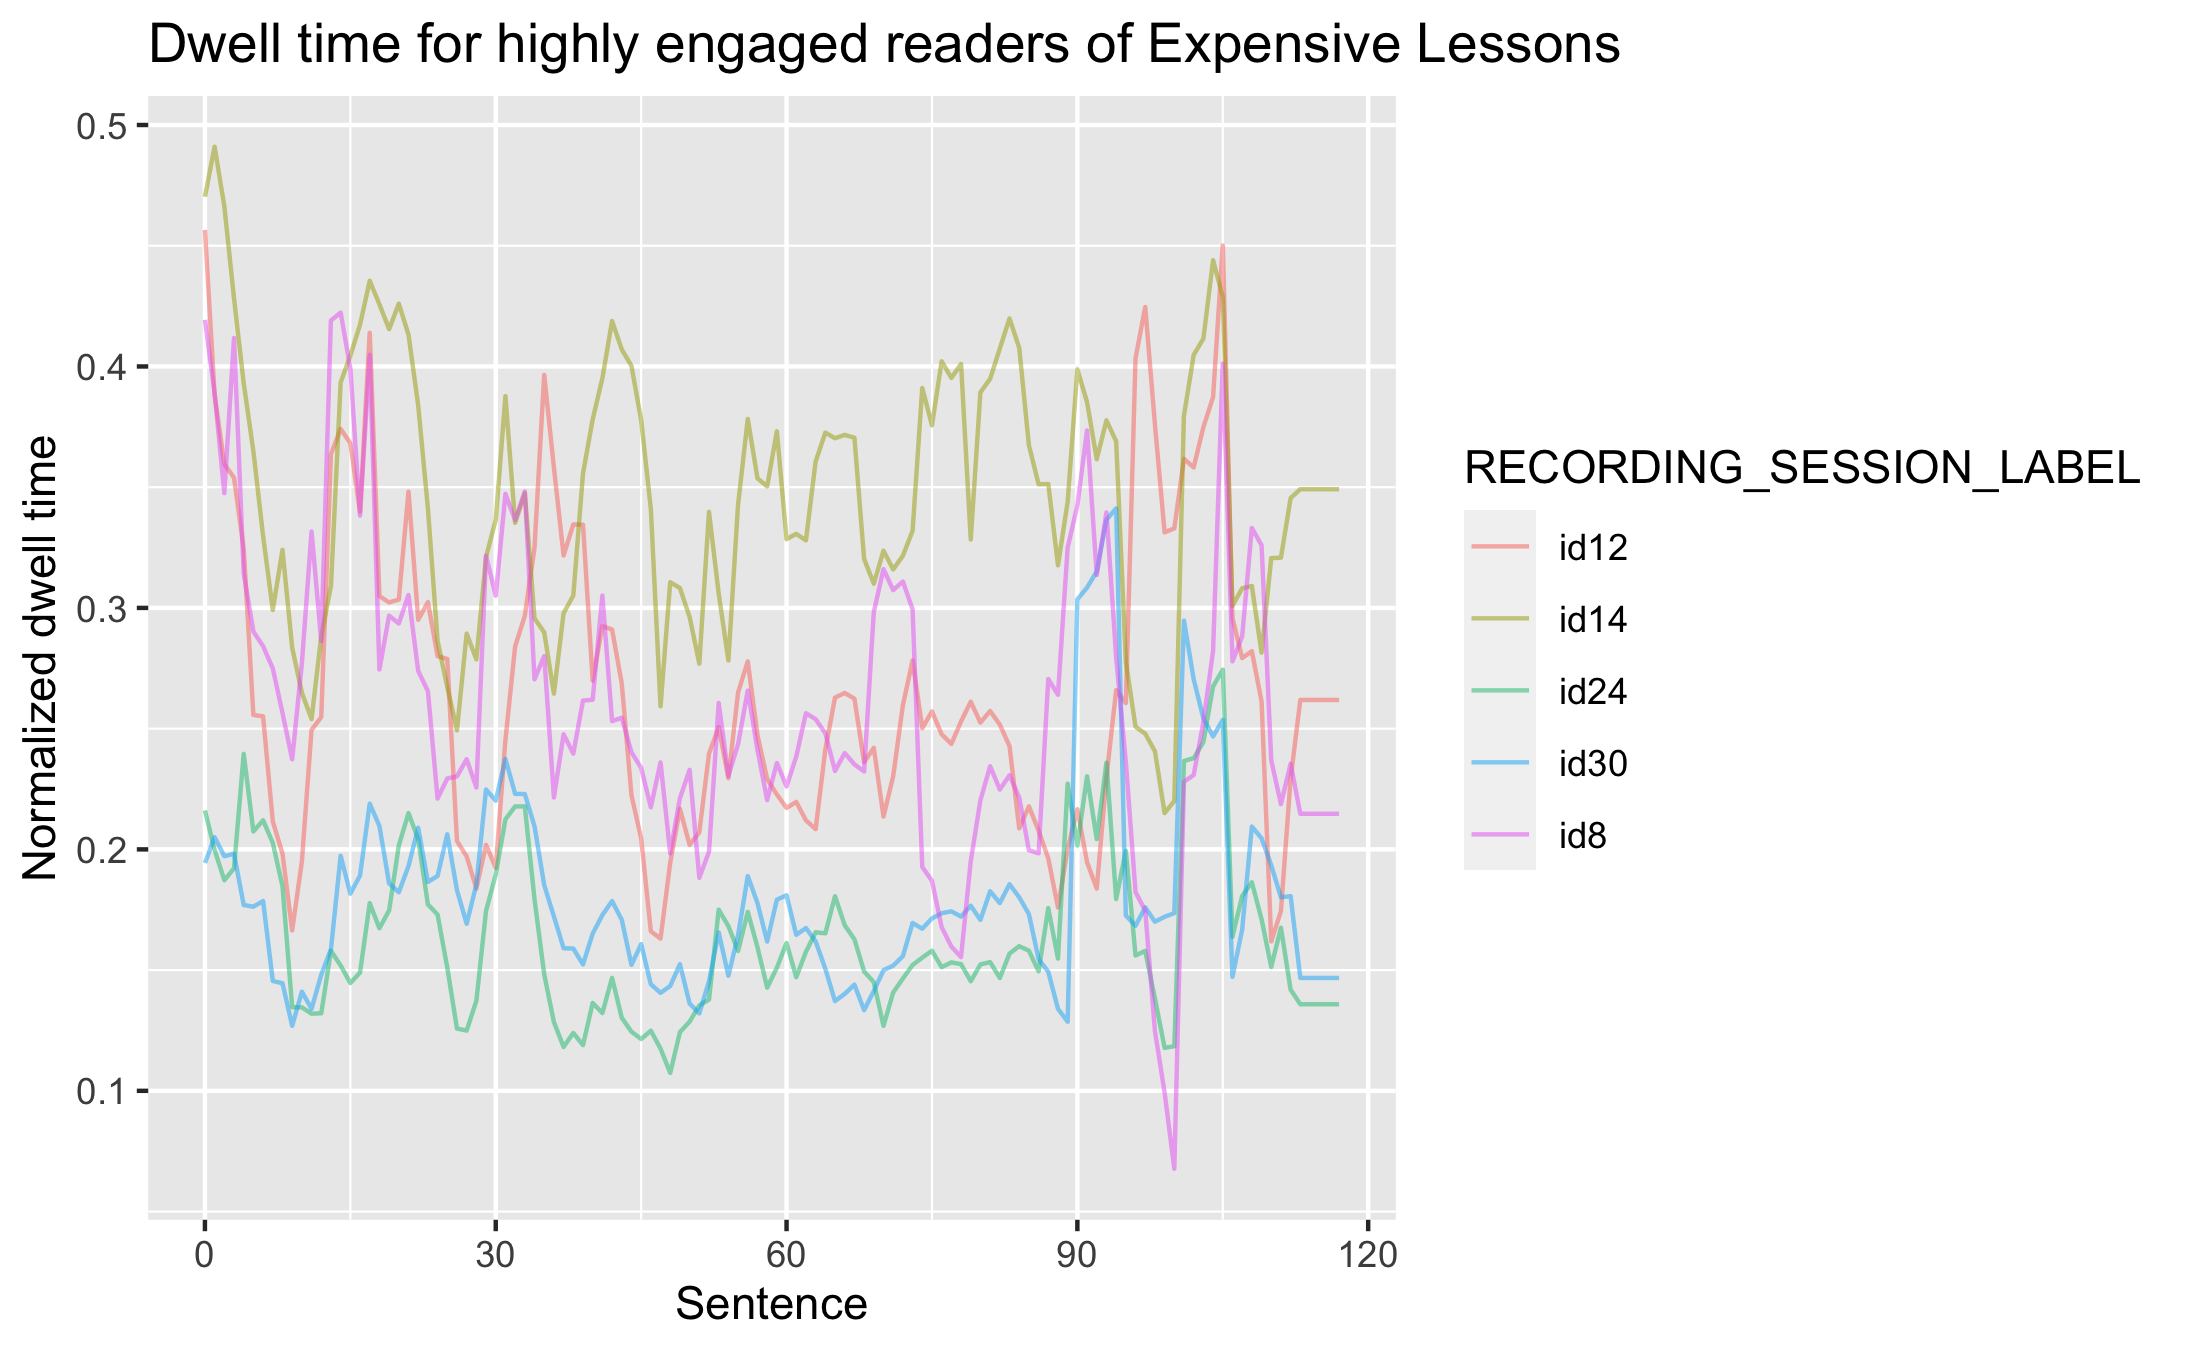
\includegraphics[height=8cm]{engaged_dt_el}
  \caption{Dwell time for engaged readers}
  \label{fig:fig2}
\end{figure*}

%\section{Future Work}


%Investigate: Does gaze duration increase in foregrounding passages and decrease in backgrounding passages?

\section{Conclusion}

By collecting reader feedback and eye tracking data on literary fiction, we were able to support findings of other studies that emphasized the importance of affective language for reader absorption. Although we found no direct relationship between dwell times and highlighted text, the dwell time model and the highlight model shared some predictors, such as valence and arousal. One possibility to explore for future studies would be to look at whether this overlap is related to two different modes of engagement --- one that leads to slower reading and one that leads to faster reading. 


\section{References}

\nocite{Green2004,liwc_22,kuzmicova2014,brysbaert2014,Maslej2019TheTF,green_brock_kaufman_2006,Consoli2018,busselle2009,jacobs2018,jacobs2017,stockwell2002cognitive,HSU201596,willems_2015,mak2019,kunze2015,ferreira-goncalo-oliveira-2018-seeking,aryani2013,delatorre2019,andrade2020,indico2015,gerrig_1993,Magyari2020,valence_arousal_dominance_2013,Brysbaert_2015}

\bibliographystyle{acl_natbib}
\bibliography{anthology,custom}


\section*{Acknowledgements}

We would like to thank the Text Group for initial feedback on experiment setup and the Blue Lantern Writing Group for additional feedback.

\end{document}